\appendix
\bibliographystyle{IEEEtran}
\bibliography{svp}

\chapter{Aditional results}



\begin{table}[H]
    \centering
    \begin{tabular}{|l|c|c|c|c|c|c|c|}
        \hline
        Model     & $AP$  & $AP@.3$ & $AP@.5$ & $AP@.75$ & $AP@.5_S$ & $AP@.5_M$ & $AP@.5_L$ \\ \hline
        YOLOv5-l6 & 0.463 & 0.869   & 0.841   & 0.442    & 0.697     & 0.887     & 0.974     \\ \hline
        EffDet-D4 & 0.297 & 0.82    & 0.735   & 0.164    & 0.552     & 0.838     & 0.815     \\ \hline
    \end{tabular}
    \caption{Comparision of trained models on the train part of stage three dataset}
    \label{tab:model_results:stage_three:train}
\end{table}

\begin{table}[H]
    \begin{tabular}{|c||c|c|c|c|}
        \hline
        Model           & Precision & Recall & F-score & $\gamma$ \\ \hline
        FRCNN-R101      & 0.69      & 0.64   & 0.664   & 0.662    \\ \hline
        FRCNN-R50       & 0.623     & 0.68   & 0.65    & 0.489    \\ \hline
        YOLOv5-m6       & 0.671     & 0.6    & 0.634   & 0.273    \\ \hline
        YOLOv5-l6       & 0.621     & 0.64   & 0.63    & 0.219    \\ \hline
        EfficientDet-D4 & 0.621     & 0.59   & 0.605   & 0.216    \\ \hline
        RetinaNet-swint & 0.661     & 0.63   & 0.645   & 0.24     \\ \hline
        RetinaNet-R50   & 0.674     & 0.6    & 0.635   & 0.41     \\ \hline
    \end{tabular}
    \caption{Precision, recall, and F-score based on the confidence threshold $\gamma$}
    \label{tab:model_prf:stage_four}
\end{table}


\begin{table}[H]
    \begin{tabular}{|c|c|c|c|c|}
        \hline
        Model           & Precision & Recall & F-score & $\gamma$ \\ \hline
        FRCNN-R101      & 0.701     & 0.67   & 0.685   & 0.664    \\ \hline
        FRCNN-R50       & 0.679     & 0.7    & 0.689   & 0.663    \\ \hline
        YOLOv5-m6       & 0.672     & 0.69   & 0.681   & 0.238    \\ \hline
        YOLOv5-l6       & 0.609     & 0.62   & 0.615   & 0.114    \\ \hline
        EfficientDet-d4 & 0.648     & 0.62   & 0.634   & 0.183    \\ \hline
        RetinaNet-swint & 0.714     & 0.67   & 0.691   & 0.401    \\ \hline
    \end{tabular}
    \caption{Precision, recall, and F-score based on the confidence threshold. Models were trained on stage-five dataset}
    \label{tab:model_prf:stage_five}
\end{table}


\begin{table}[H]
    \centering
    \begin{tabular}{|c|c|c|c|c|c|c|c|}
        \hline
        Model      & $AR$  & $AR@.5_{10}$ & $AR@.5$ & $AR@.75$ & $AR@.5_S$ & $AR@.5_M$ & $AR@.5_L$ \\ \hline
        YOLOv5-l6  & 0.559 & 0.895        & 0.956   & 0.559    & 0.916     & 0.971     & 0.971     \\ \hline
        YOLOv5-m6  & 0.547 & 0.899        & 0.957   & 0.541    & 0.933     & 0.971     & 0.971     \\ \hline
        YOLOv5-s6  & 0.545 & 0.877        & 0.951   & 0.549    & 0.916     & 0.968     & 0.968     \\ \hline
        Effdet-D1  & 0.531 & 0.87         & 0.958   & 0.488    & 0.909     & 0.978     & 0.978     \\ \hline
        FRCNN-R50  & 0.475 & 0.867        & 0.883   & 0.445    & 0.832     & 0.899     & 0.899     \\ \hline
        FRCNN-R101 & 0.478 & 0.864        & 0.89    & 0.458    & 0.815     & 0.917     & 0.917     \\ \hline
        RetN-swint & 0.508 & 0.89         & 0.946   & 0.468    & 0.902     & 0.967     & 0.967     \\ \hline
    \end{tabular}
    \caption{Average racall of improved models}
    \label{tab:improved:recall}
\end{table}


\begin{table}[H]
    \begin{tabular}{|c|c|c|c|c|}
        \hline
        Model      & Precision & Recall & F-score & Confidence threshold \\ \hline
        YOLOv5-l6  & 0.689     & 0.69   & 0.689   & 0.271                \\ \hline
        YOLOv5-m6  & 0.74      & 0.64   & 0.686   & 0.326                \\ \hline
        YOLOv5-s6  & 0.692     & 0.64   & 0.665   & 0.295                \\ \hline
        Effdet-D1  & 0.739     & 0.64   & 0.686   & 0.339                \\ \hline
        FRCNN-R50  & 0.719     & 0.66   & 0.688   & 0.759                \\ \hline
        FRCNN-R101 & 0.704     & 0.63   & 0.665   & 0.684                \\ \hline
        RetN-swint & 0.681     & 0.69   & 0.685   & 0.367                \\ \hline
    \end{tabular}
    \caption{Precision, recall, and F-score based on the confidence threshold for different models}
    \label{tab:imrpoved:prf}
\end{table}

\begin{table}[h]
    \centering
    \begin{tabular}{|c|c|c|c|c|c|c|c|}
        \hline
        Method & $AR$  & $AR@.5_{10}$ & $AR@.5$ & $AR@.75$ & $AR@.5_S$ & $AR@.5_M$ & $AR@.5_L$ \\ \hline
        NMS    & 0.546 & 0.91         & 0.971   & 0.522    & 0.949     & 0.98      & 0.98      \\ \hline
        S-NMS  & 0.584 & 0.888        & 0.951   & 0.603    & 0.912     & 0.965     & 0.965     \\ \hline
        NWM    & 0.526 & 0.913        & 0.941   & 0.513    & 0.892     & 0.959     & 0.959     \\ \hline
        WBF    & 0.573 & 0.918        & 0.975   & 0.569    & 0.956     & 0.981     & 0.981     \\ \hline
        WBF-A  & 0.572 & 0.92         & 0.974   & 0.566    & 0.956     & 0.98      & 0.98      \\ \hline
    \end{tabular}
    \caption{Average recall of models ensembled by parameters from table \ref{tab:ensemble_params:grid_search}}
    \label{tab:recall:grid_search}
\end{table}


\begin{table}[h]
    \begin{tabular}{|c|c|c|c|c|}
        \hline
        Method & Precision & Recall & F-score & Confidence threshold \\ \hline
        NMS    & 0.708     & 0.68   & 0.694   & 0.284                \\ \hline
        S-NMS  & 0.679     & 0.7    & 0.689   & 0.489                \\ \hline
        NWM    & 0.713     & 0.71   & 0.712   & 0.792                \\ \hline
        WBF    & 0.732     & 0.7    & 0.715   & 0.594                \\ \hline
        WBF-A  & 0.745     & 0.69   & 0.716   & 0.201                \\ \hline
    \end{tabular}
    \caption{Precision, recall, and F-score based on the confidence threshold for different ensembling methods}
    \label{tab:ensembling_prf:grid_search}
\end{table}

\section{Detection of detnal caries and segmentation of dental restorations}
\begin{figure}[h]
    \centering
    \begin{subfigure}[b]{0.9\textwidth}
        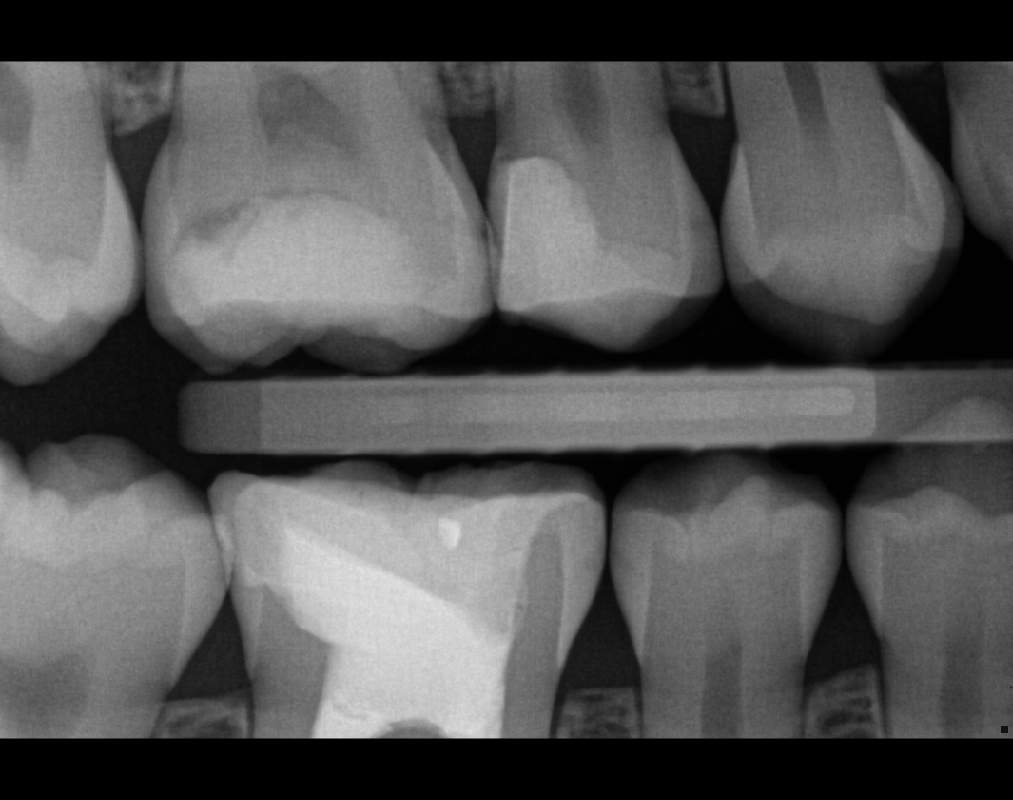
\includegraphics[width=1\linewidth]{images/det1orig.png}
        % \caption{}
    \end{subfigure}

    \begin{subfigure}[b]{0.9\textwidth}
        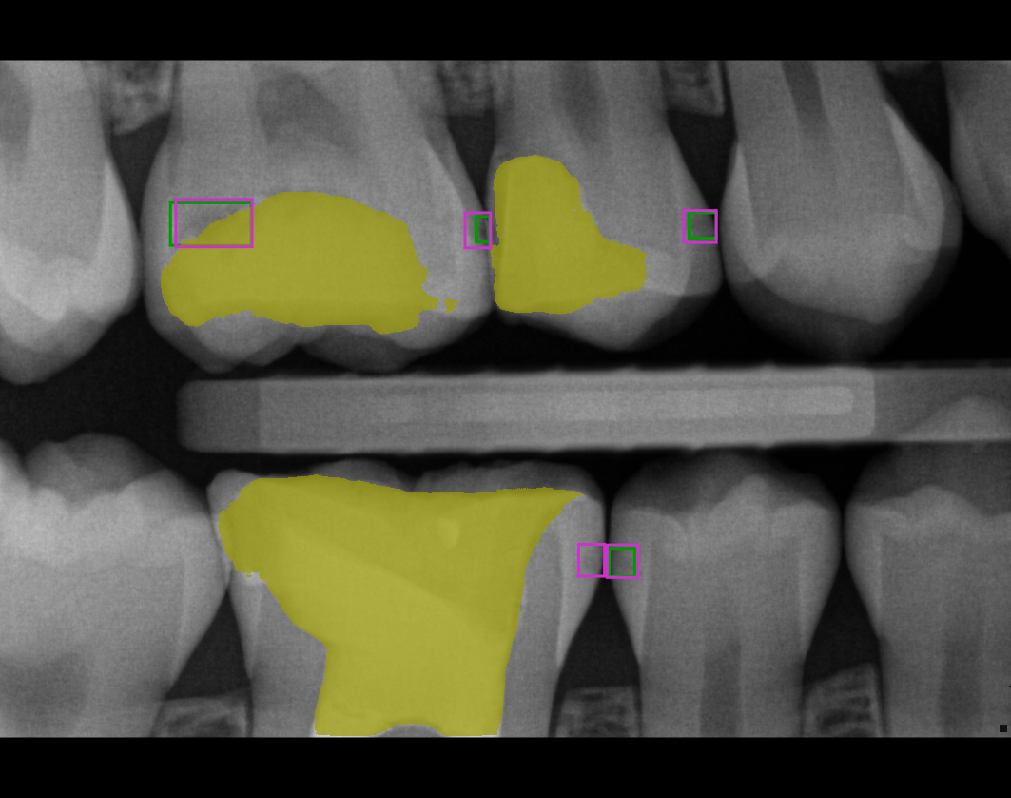
\includegraphics[width=1\linewidth]{images/det1pred.png}
        % \caption{}
    \end{subfigure}
    % \caption{}
    % \label{}
\end{figure}


\begin{figure}[h]
    \centering
    \begin{subfigure}[b]{0.9\textwidth}
        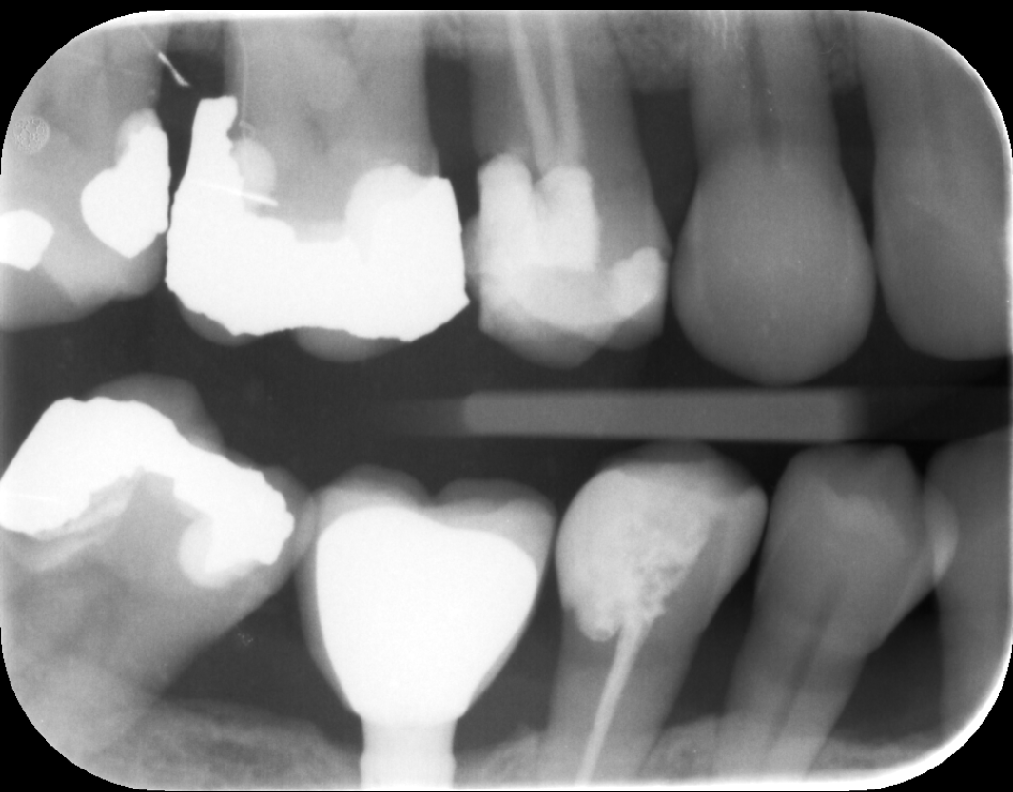
\includegraphics[width=1\linewidth]{images/det2orig.png}
        \caption{Original image}
    \end{subfigure}

    \begin{subfigure}[b]{0.9\textwidth}
        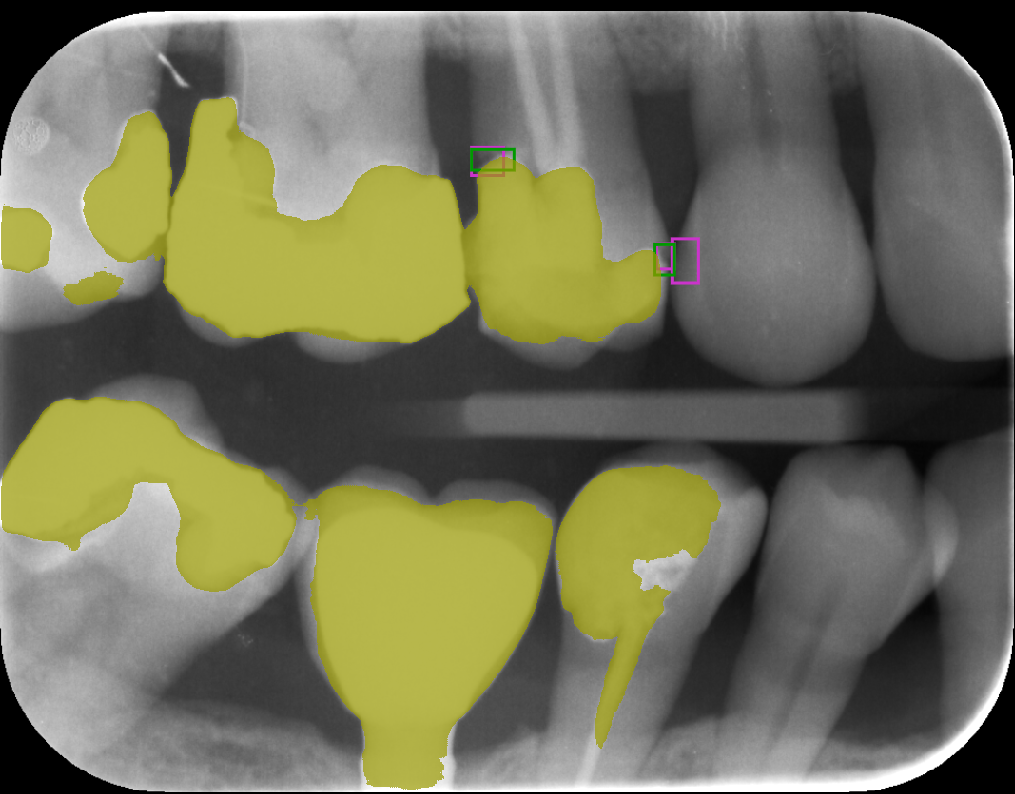
\includegraphics[width=1\linewidth]{images/det2pred.png}
        \caption{Output of our models}
    \end{subfigure}
    \caption{ Segmented dental restorations in yellow, predicted dental caries are pink and ground truth of dental caries in green. We see a single false pasitive detection on the top right of the image}
    \label{}
\end{figure}

\chapter{Images}
\label{appendix:model_predictions}
\section{Predictions of the model}
The following figures are X-ray images from the test part of dataset. Ground truth labels are marked by pink color and the model predictions are in green. Each bounding box prediction has corresponging confidence attached to it.
\begin{figure}[H]
    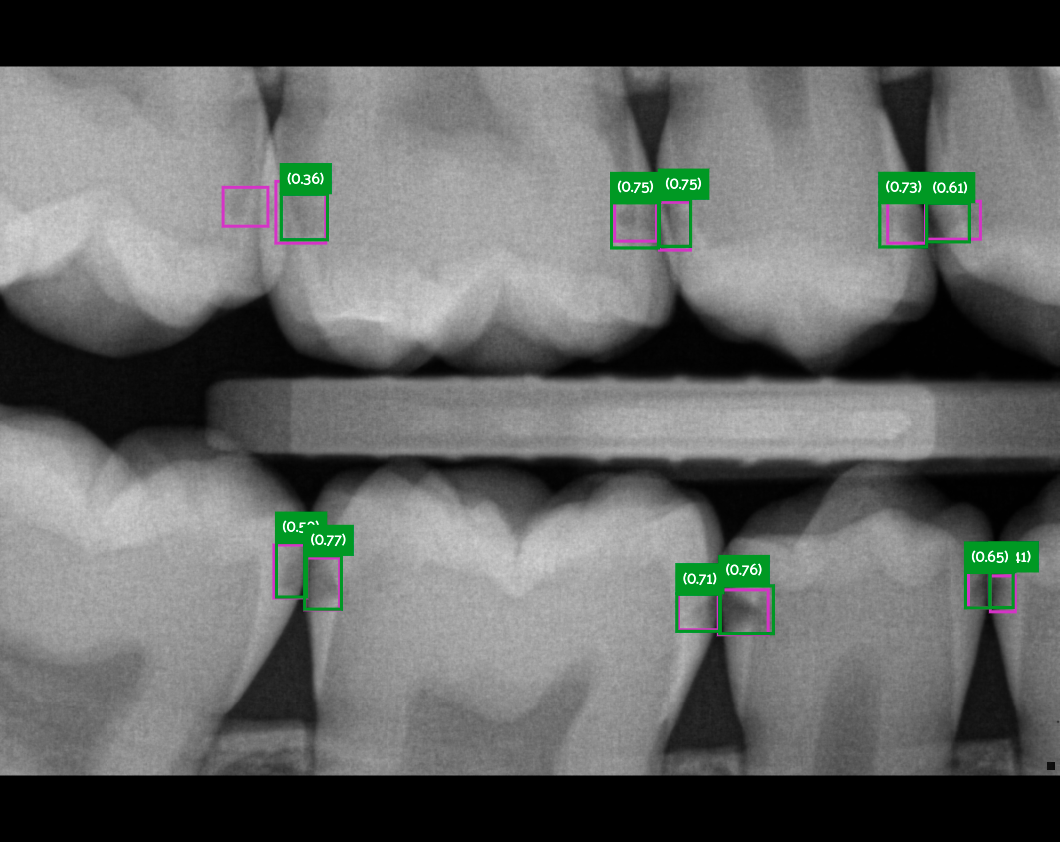
\includegraphics[width=0.9\linewidth]{images/no_rest1.png}
    \caption{X-ray image with ground truth boxes and model's predictions}
    \label{fig:pred_img1}
\end{figure}

\begin{figure}[H]
    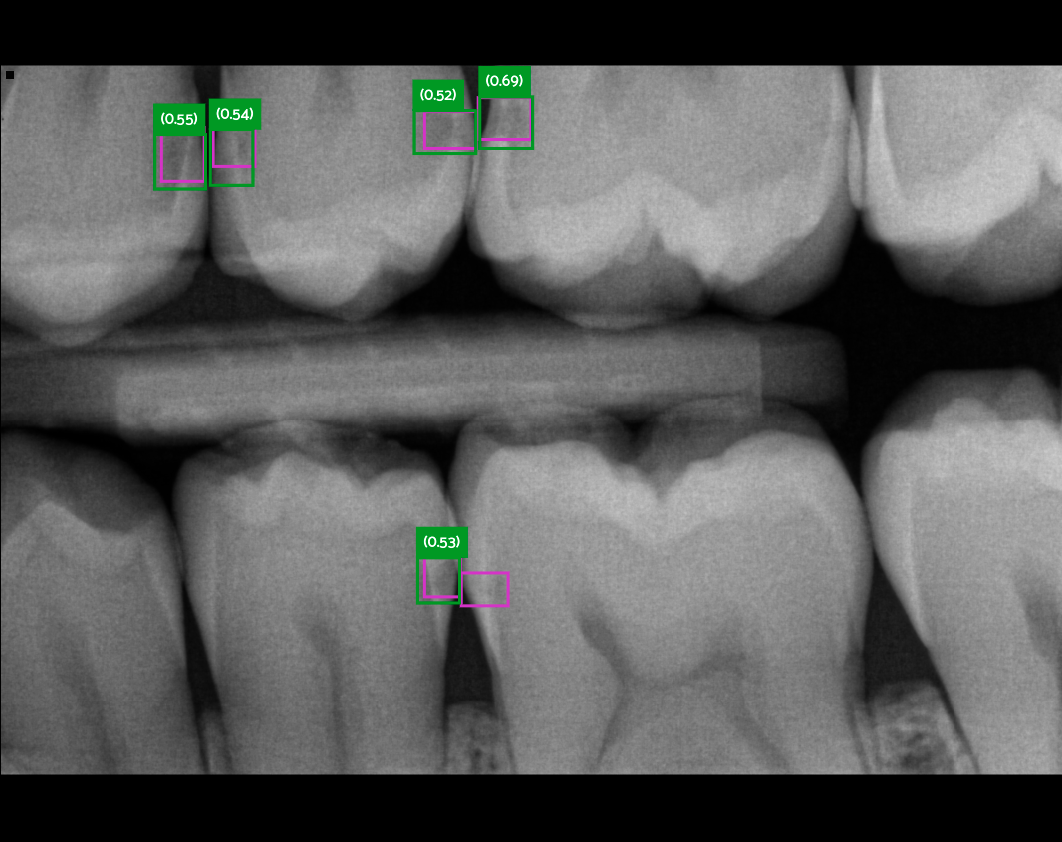
\includegraphics[width=0.9\linewidth]{images/no_rest2.png}
    \caption{X-ray image with ground truth boxes and model's predictions}
    \label{fig:pred_img2}
\end{figure}

\begin{figure}[H]
    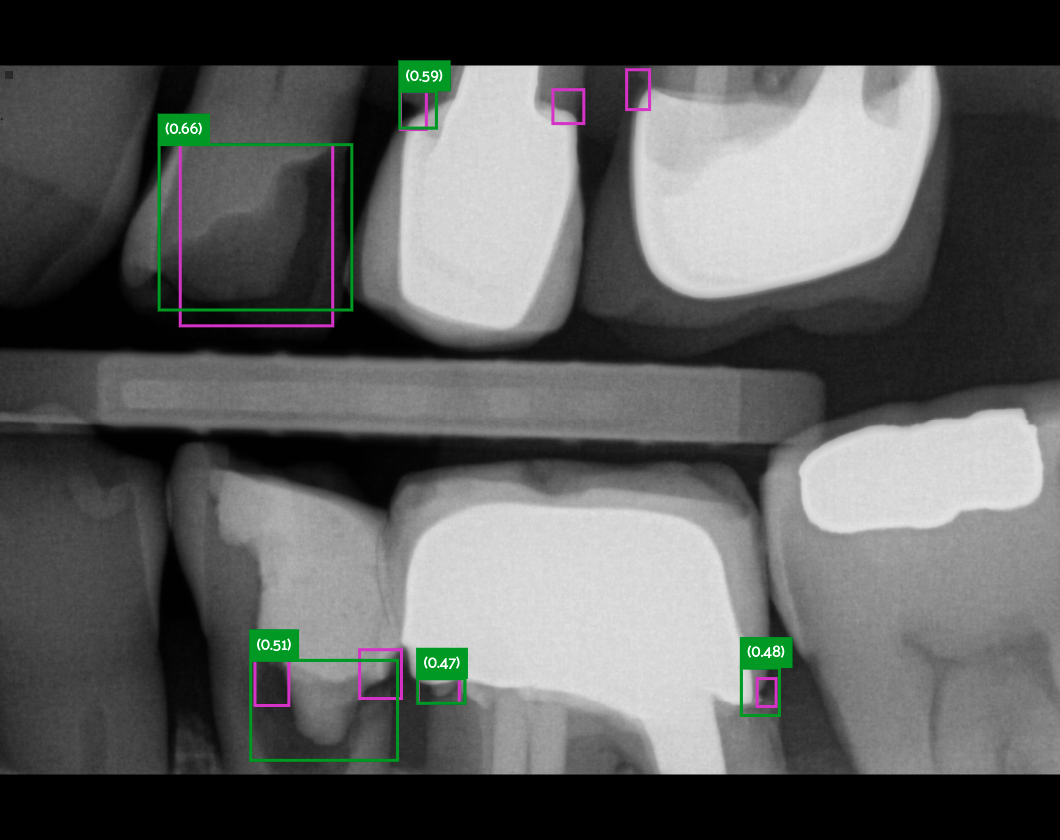
\includegraphics[width=0.9\linewidth]{images/rest1.png}
    \caption{X-ray image with ground truth boxes and model's predictions}
    \label{fig:pred_img3}
\end{figure}

\begin{figure}[H]
    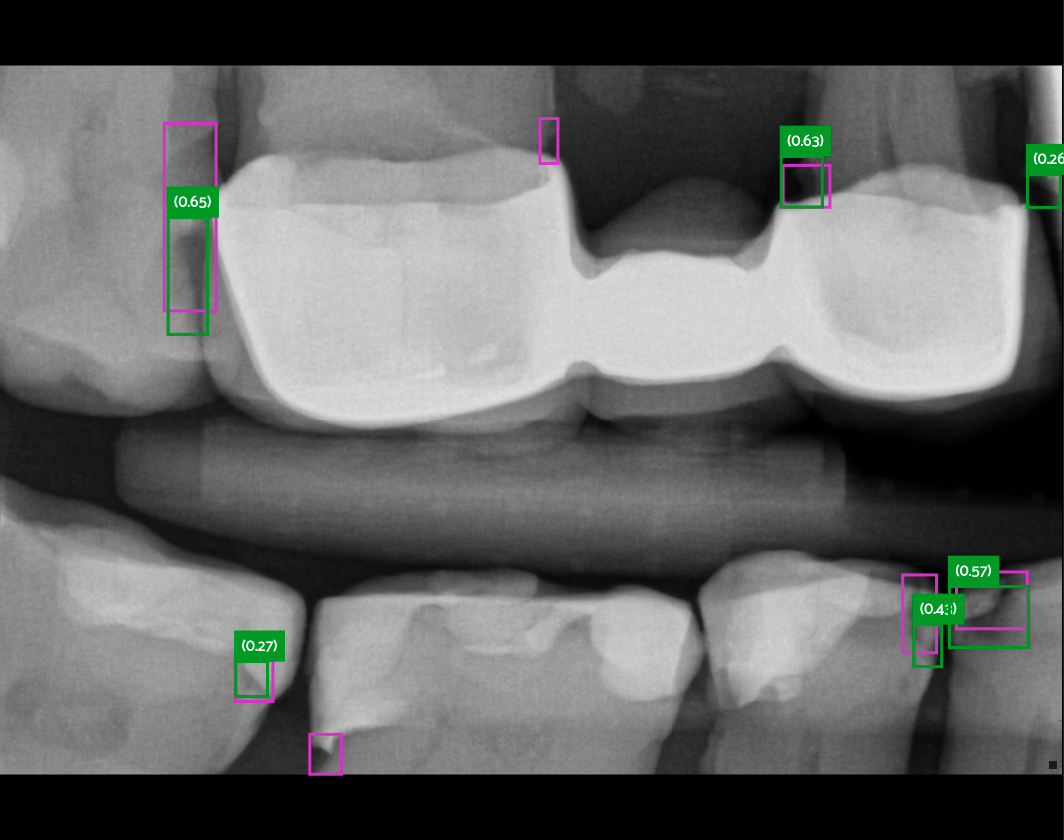
\includegraphics[width=0.9\linewidth]{images/rest2.png}
    \caption{X-ray image with ground truth boxes and model's predictions}
    \label{fig:pred_img4}
\end{figure}

% \chapter{Model importance during ensembling}
\section{Model importance during ensembling}


\begin{figure}[H]
    \centering
    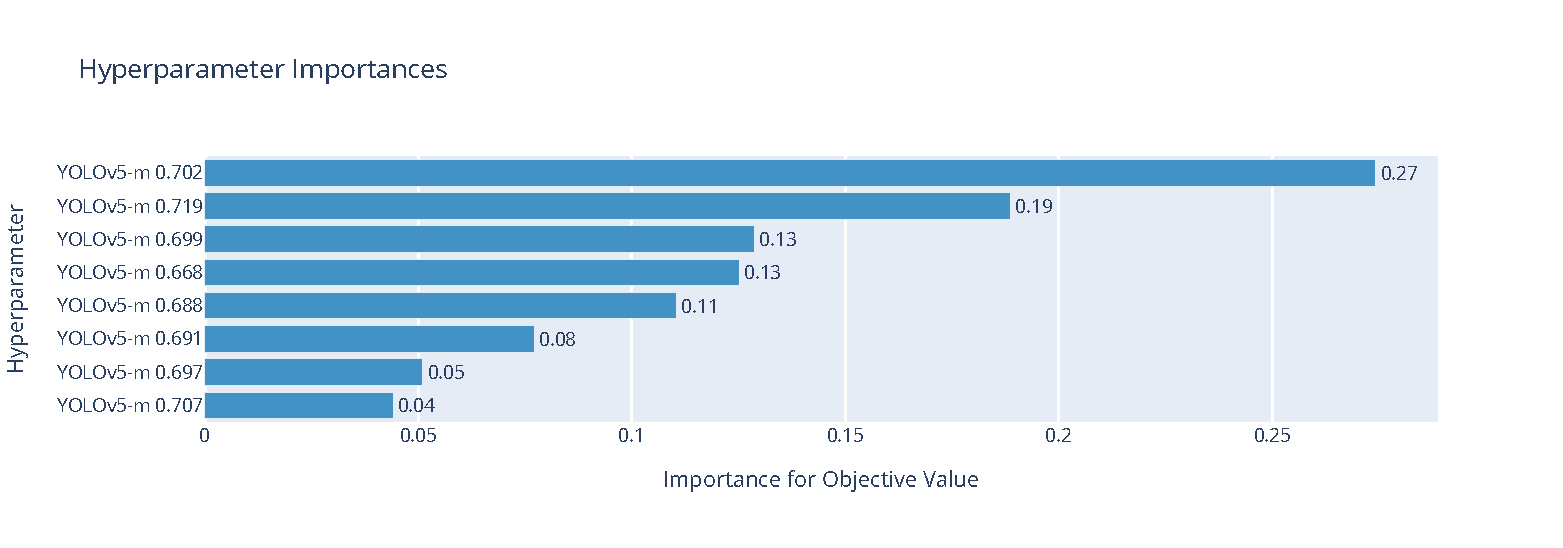
\includegraphics[width=\linewidth]{images/ensemble_yolo_importance.pdf}
    \caption{Importance of different models during ensembling with the same architectures and backbones}
    \label{fig:ensembling_hparams_imprtance_yolo_m}
\end{figure}

\begin{figure}[H]
    \centering
    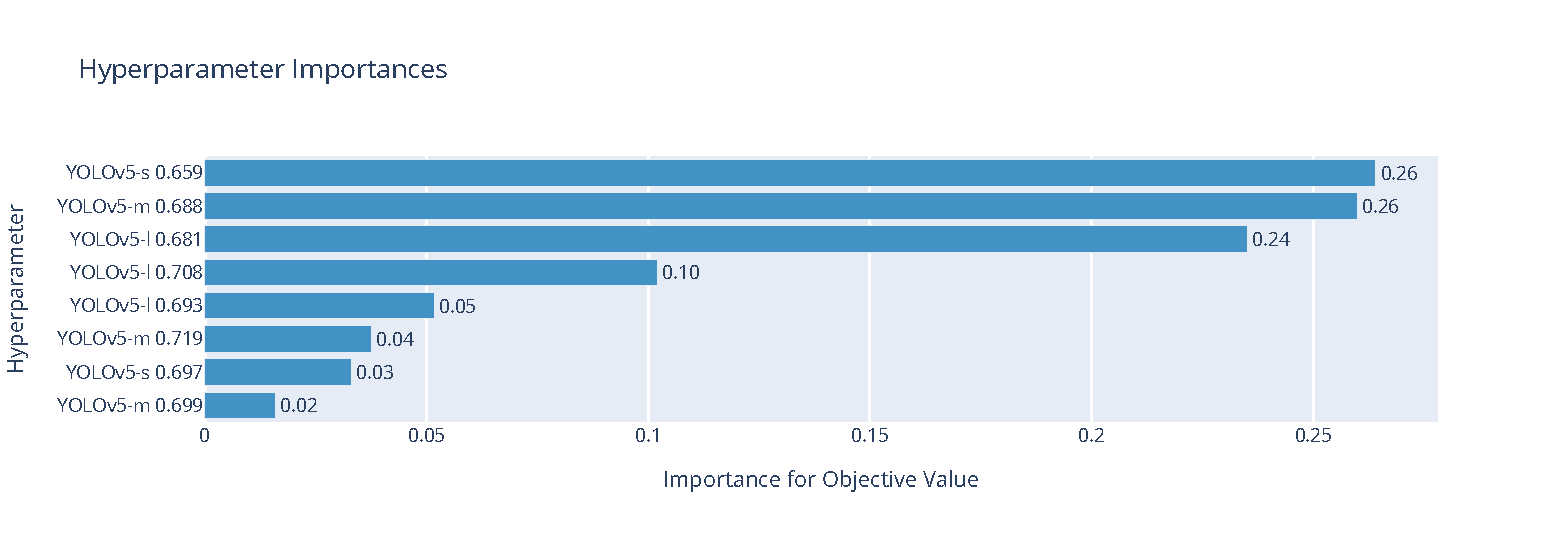
\includegraphics[width=\linewidth]{images/ensemble_yolo_mix_importance.pdf}
    \caption{Importance of different models during ensembling with the architecture and different backbones}
    \label{fig:ensembling_hparams_imprtance_yolo_mix}
\end{figure}

% \chapter{Augmented images}
\section{Augmented images}
\label{appendix:img_transformations}
\begin{figure}
    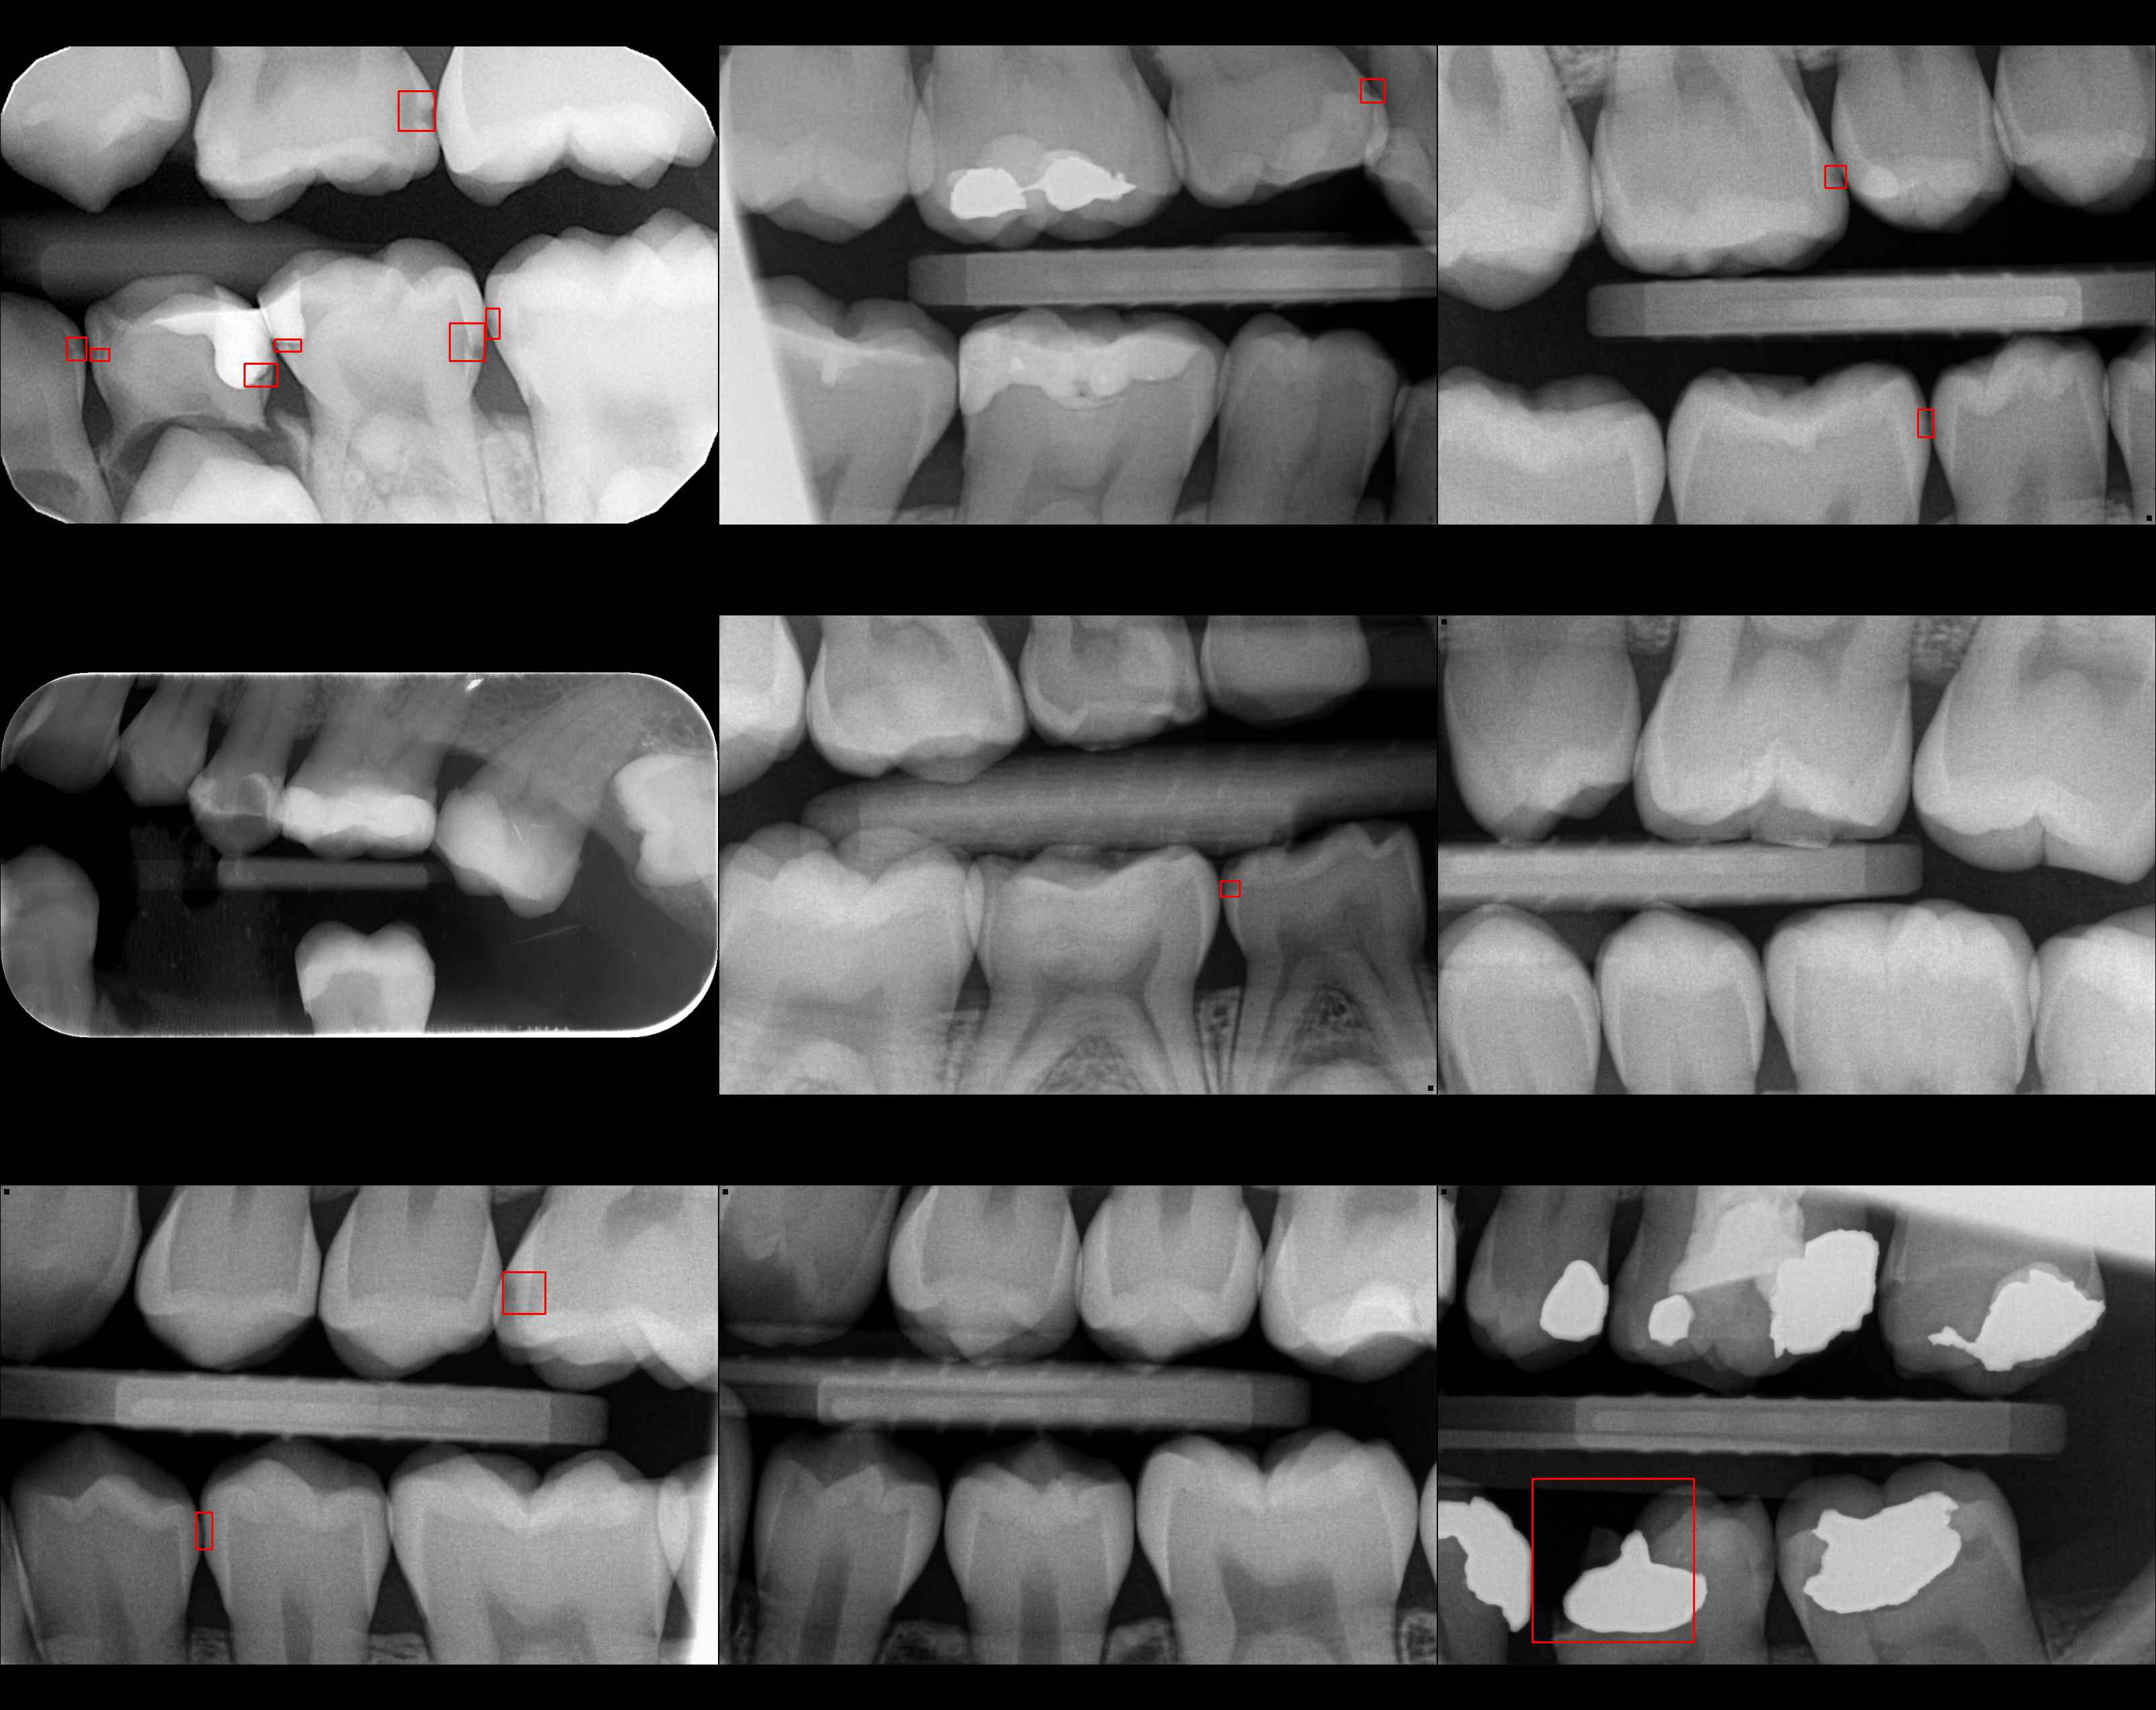
\includegraphics[width =0.8\linewidth]{images/no_trasnforms.jpg}
    \caption{No transformation applied}
\end{figure}
\begin{figure}
    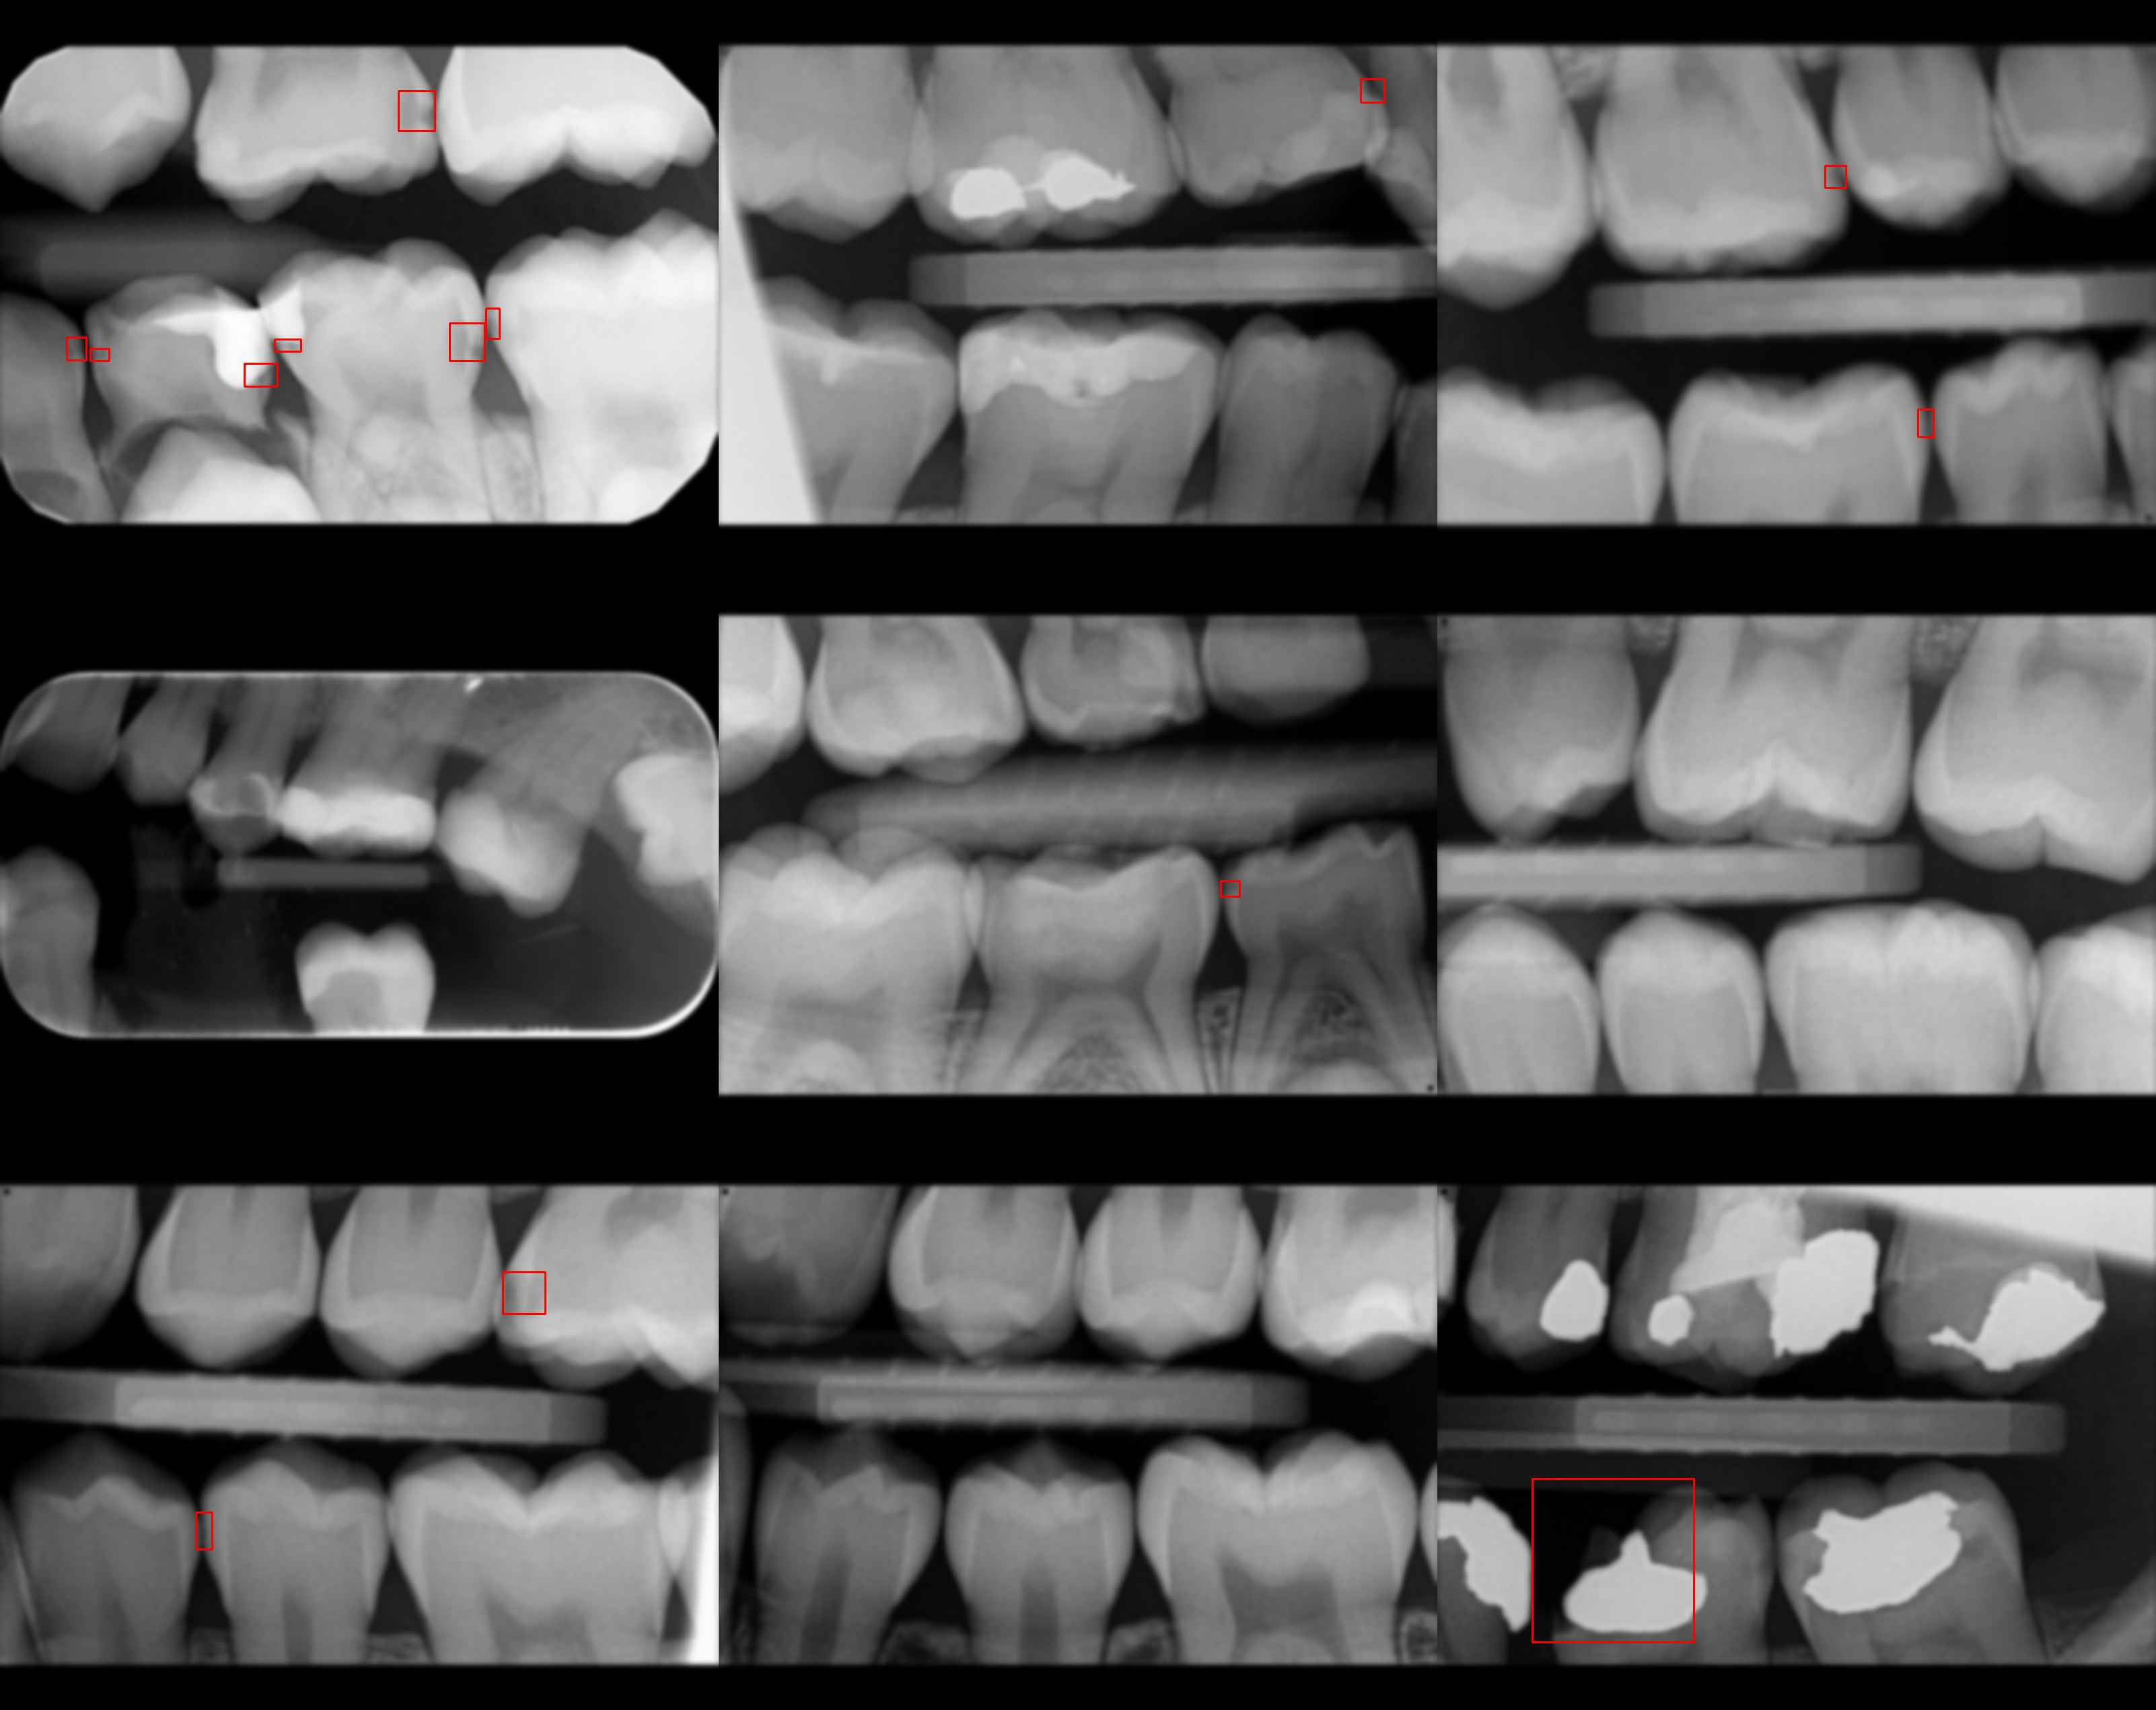
\includegraphics[width =0.8\linewidth]{images/gaussian_blur.jpg}
    \caption{Gaussian blur applied}
\end{figure}
\begin{figure}
    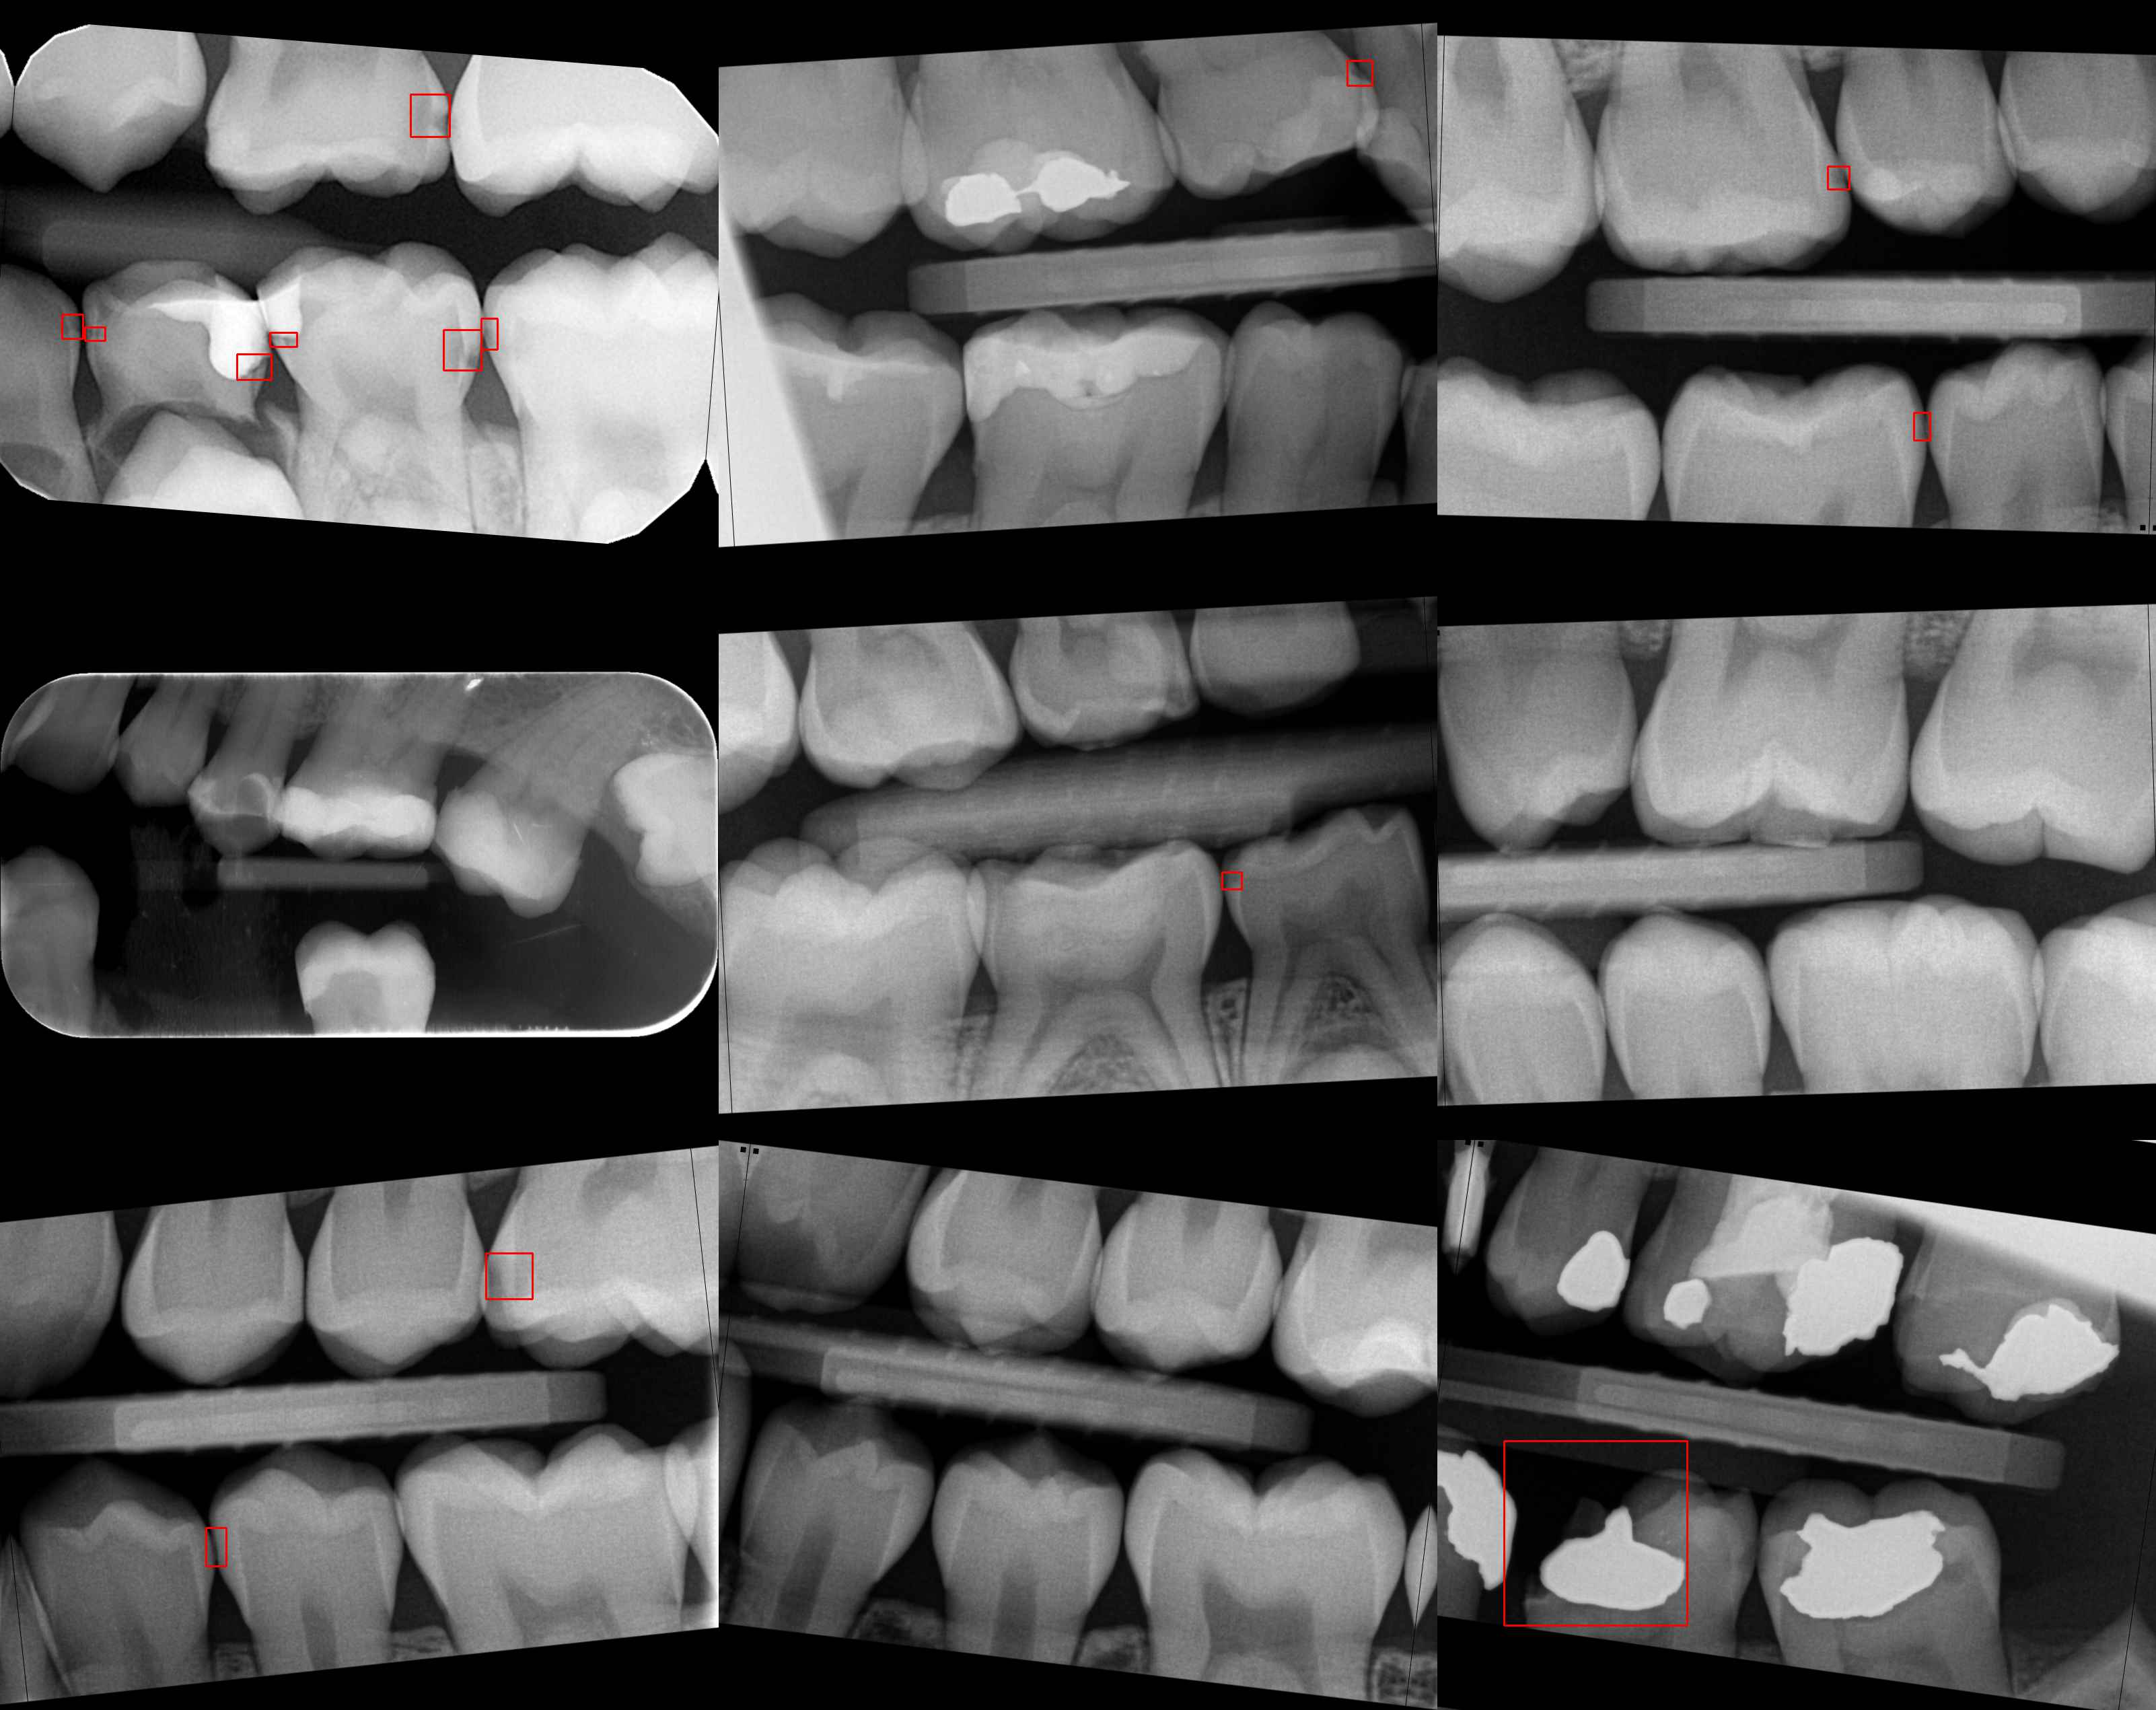
\includegraphics[width =0.8\linewidth]{images/roate_10.jpg}
    \caption{Rotation applied}
\end{figure}
\begin{figure}
    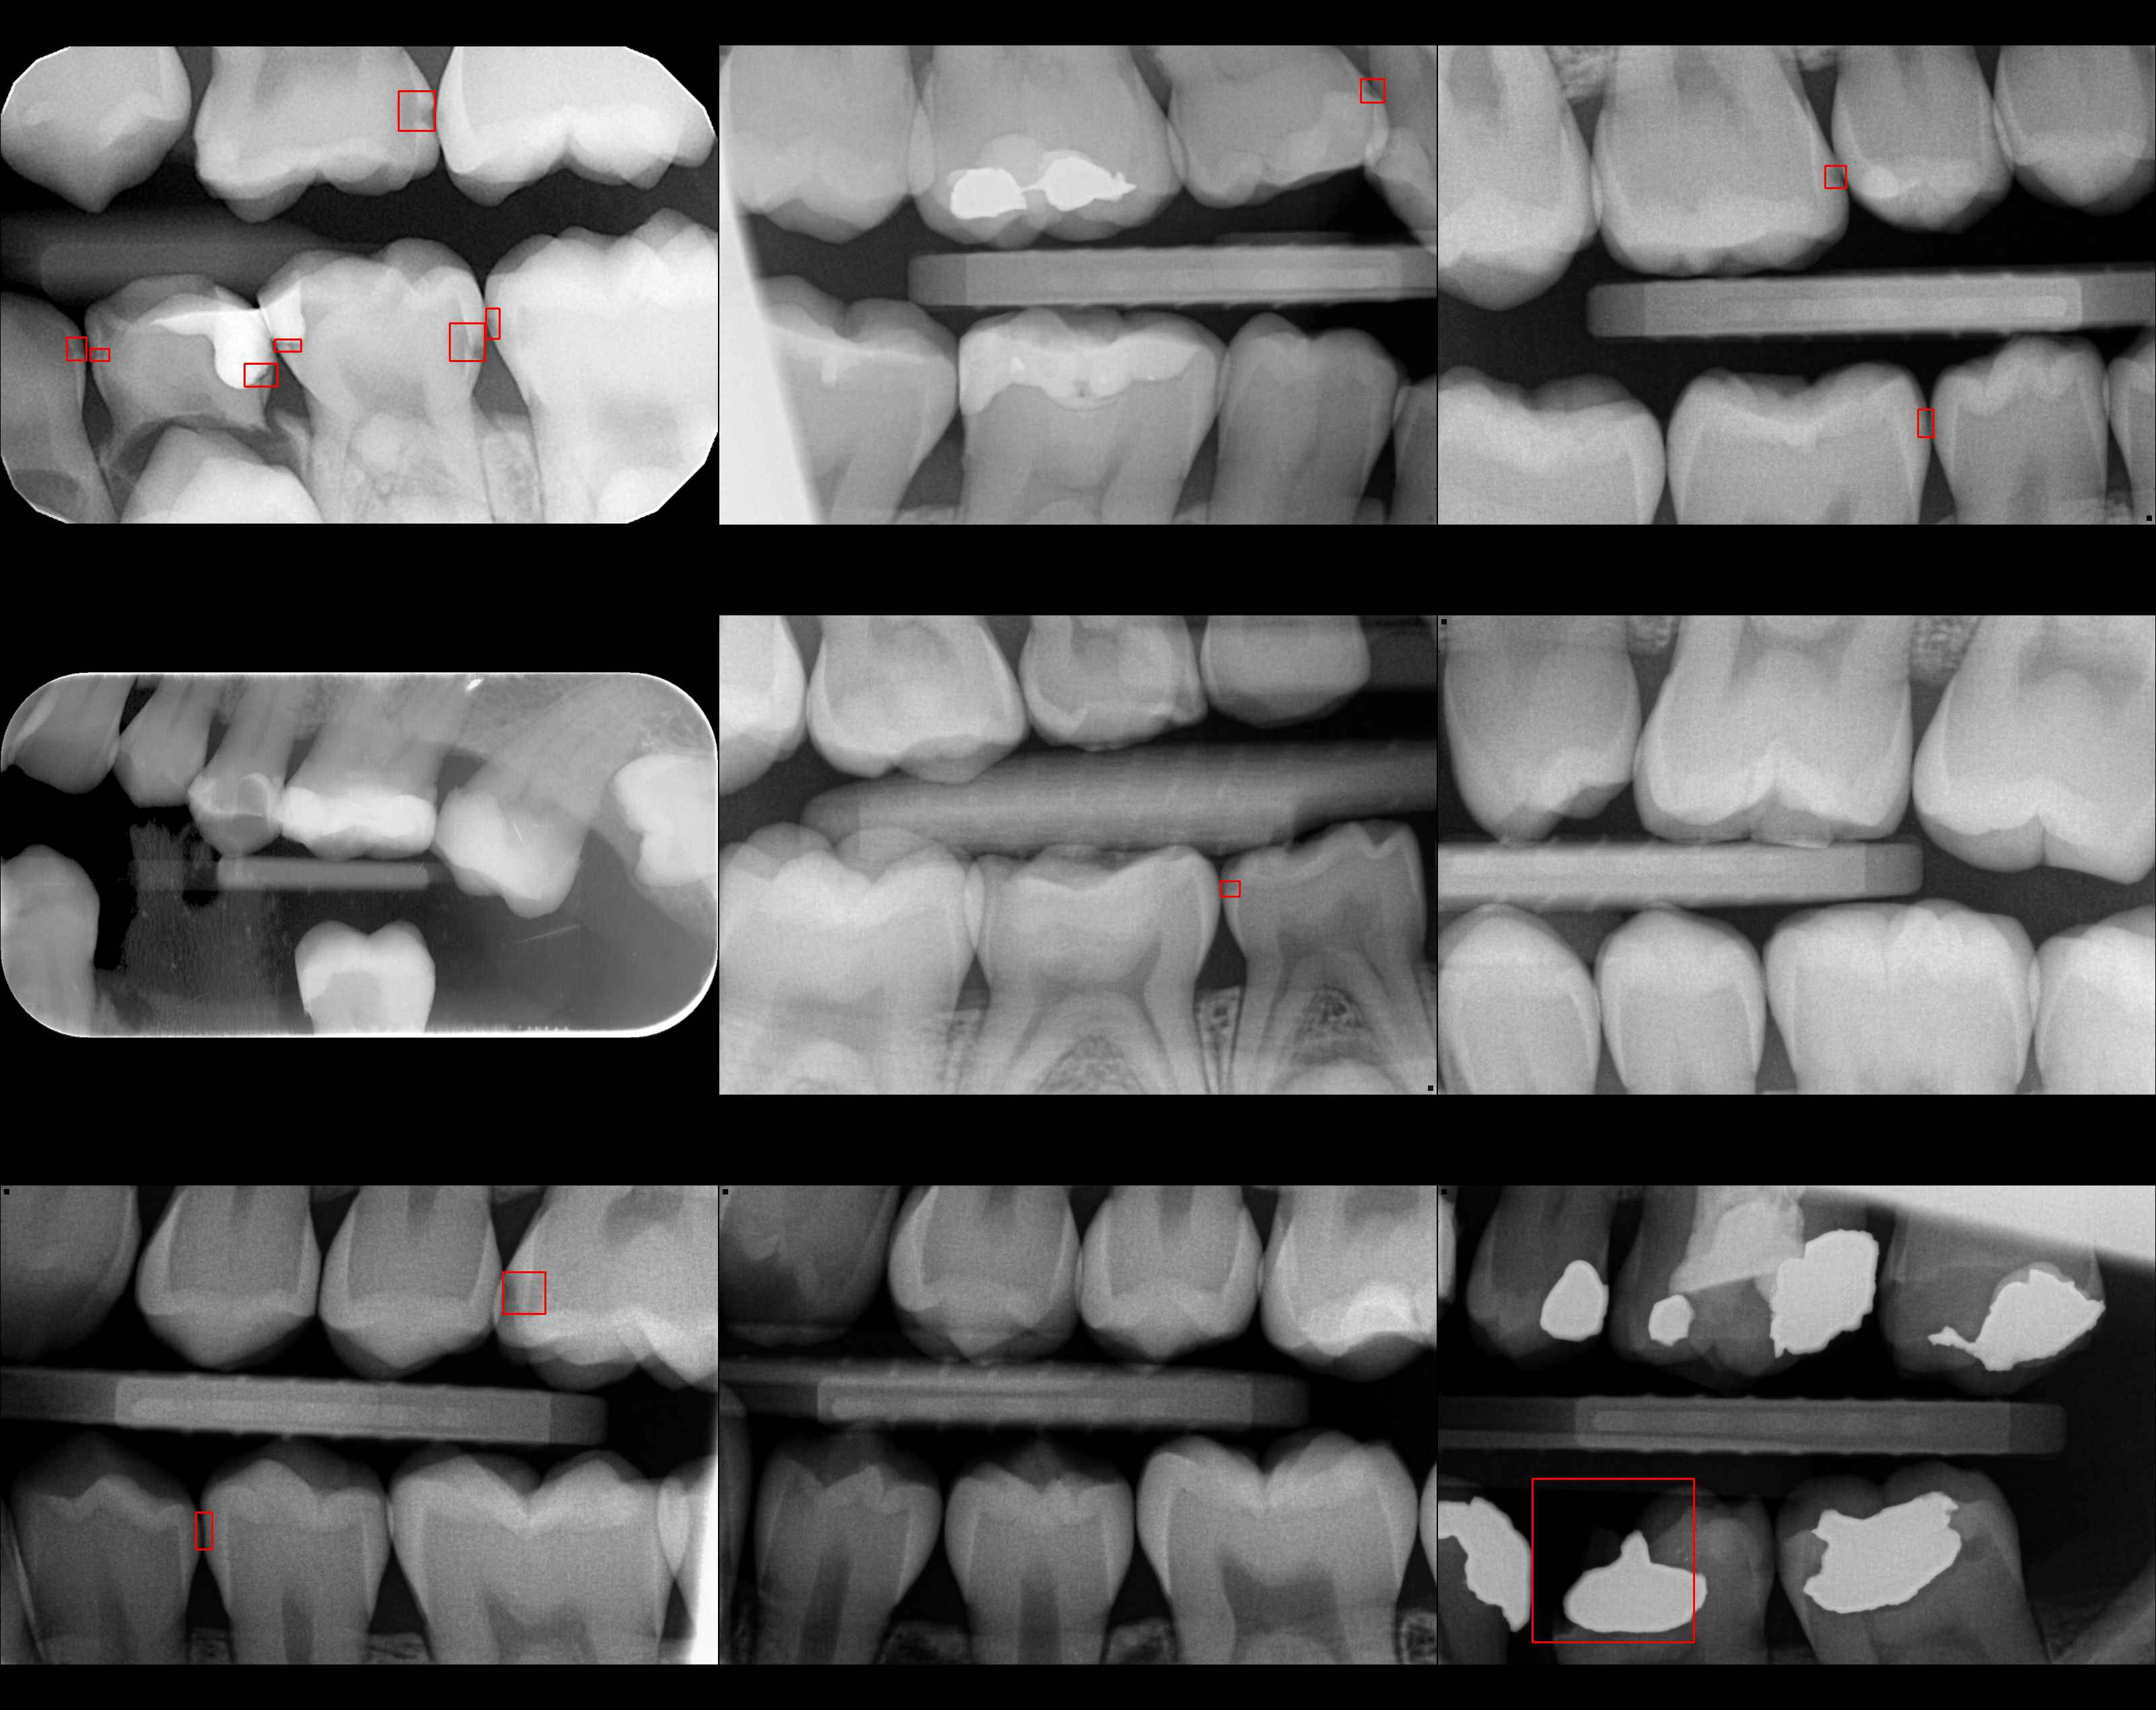
\includegraphics[width =0.8\linewidth]{images/random_gamma.jpg}
    \caption{Gamma correction applied}
\end{figure}
\begin{figure}
    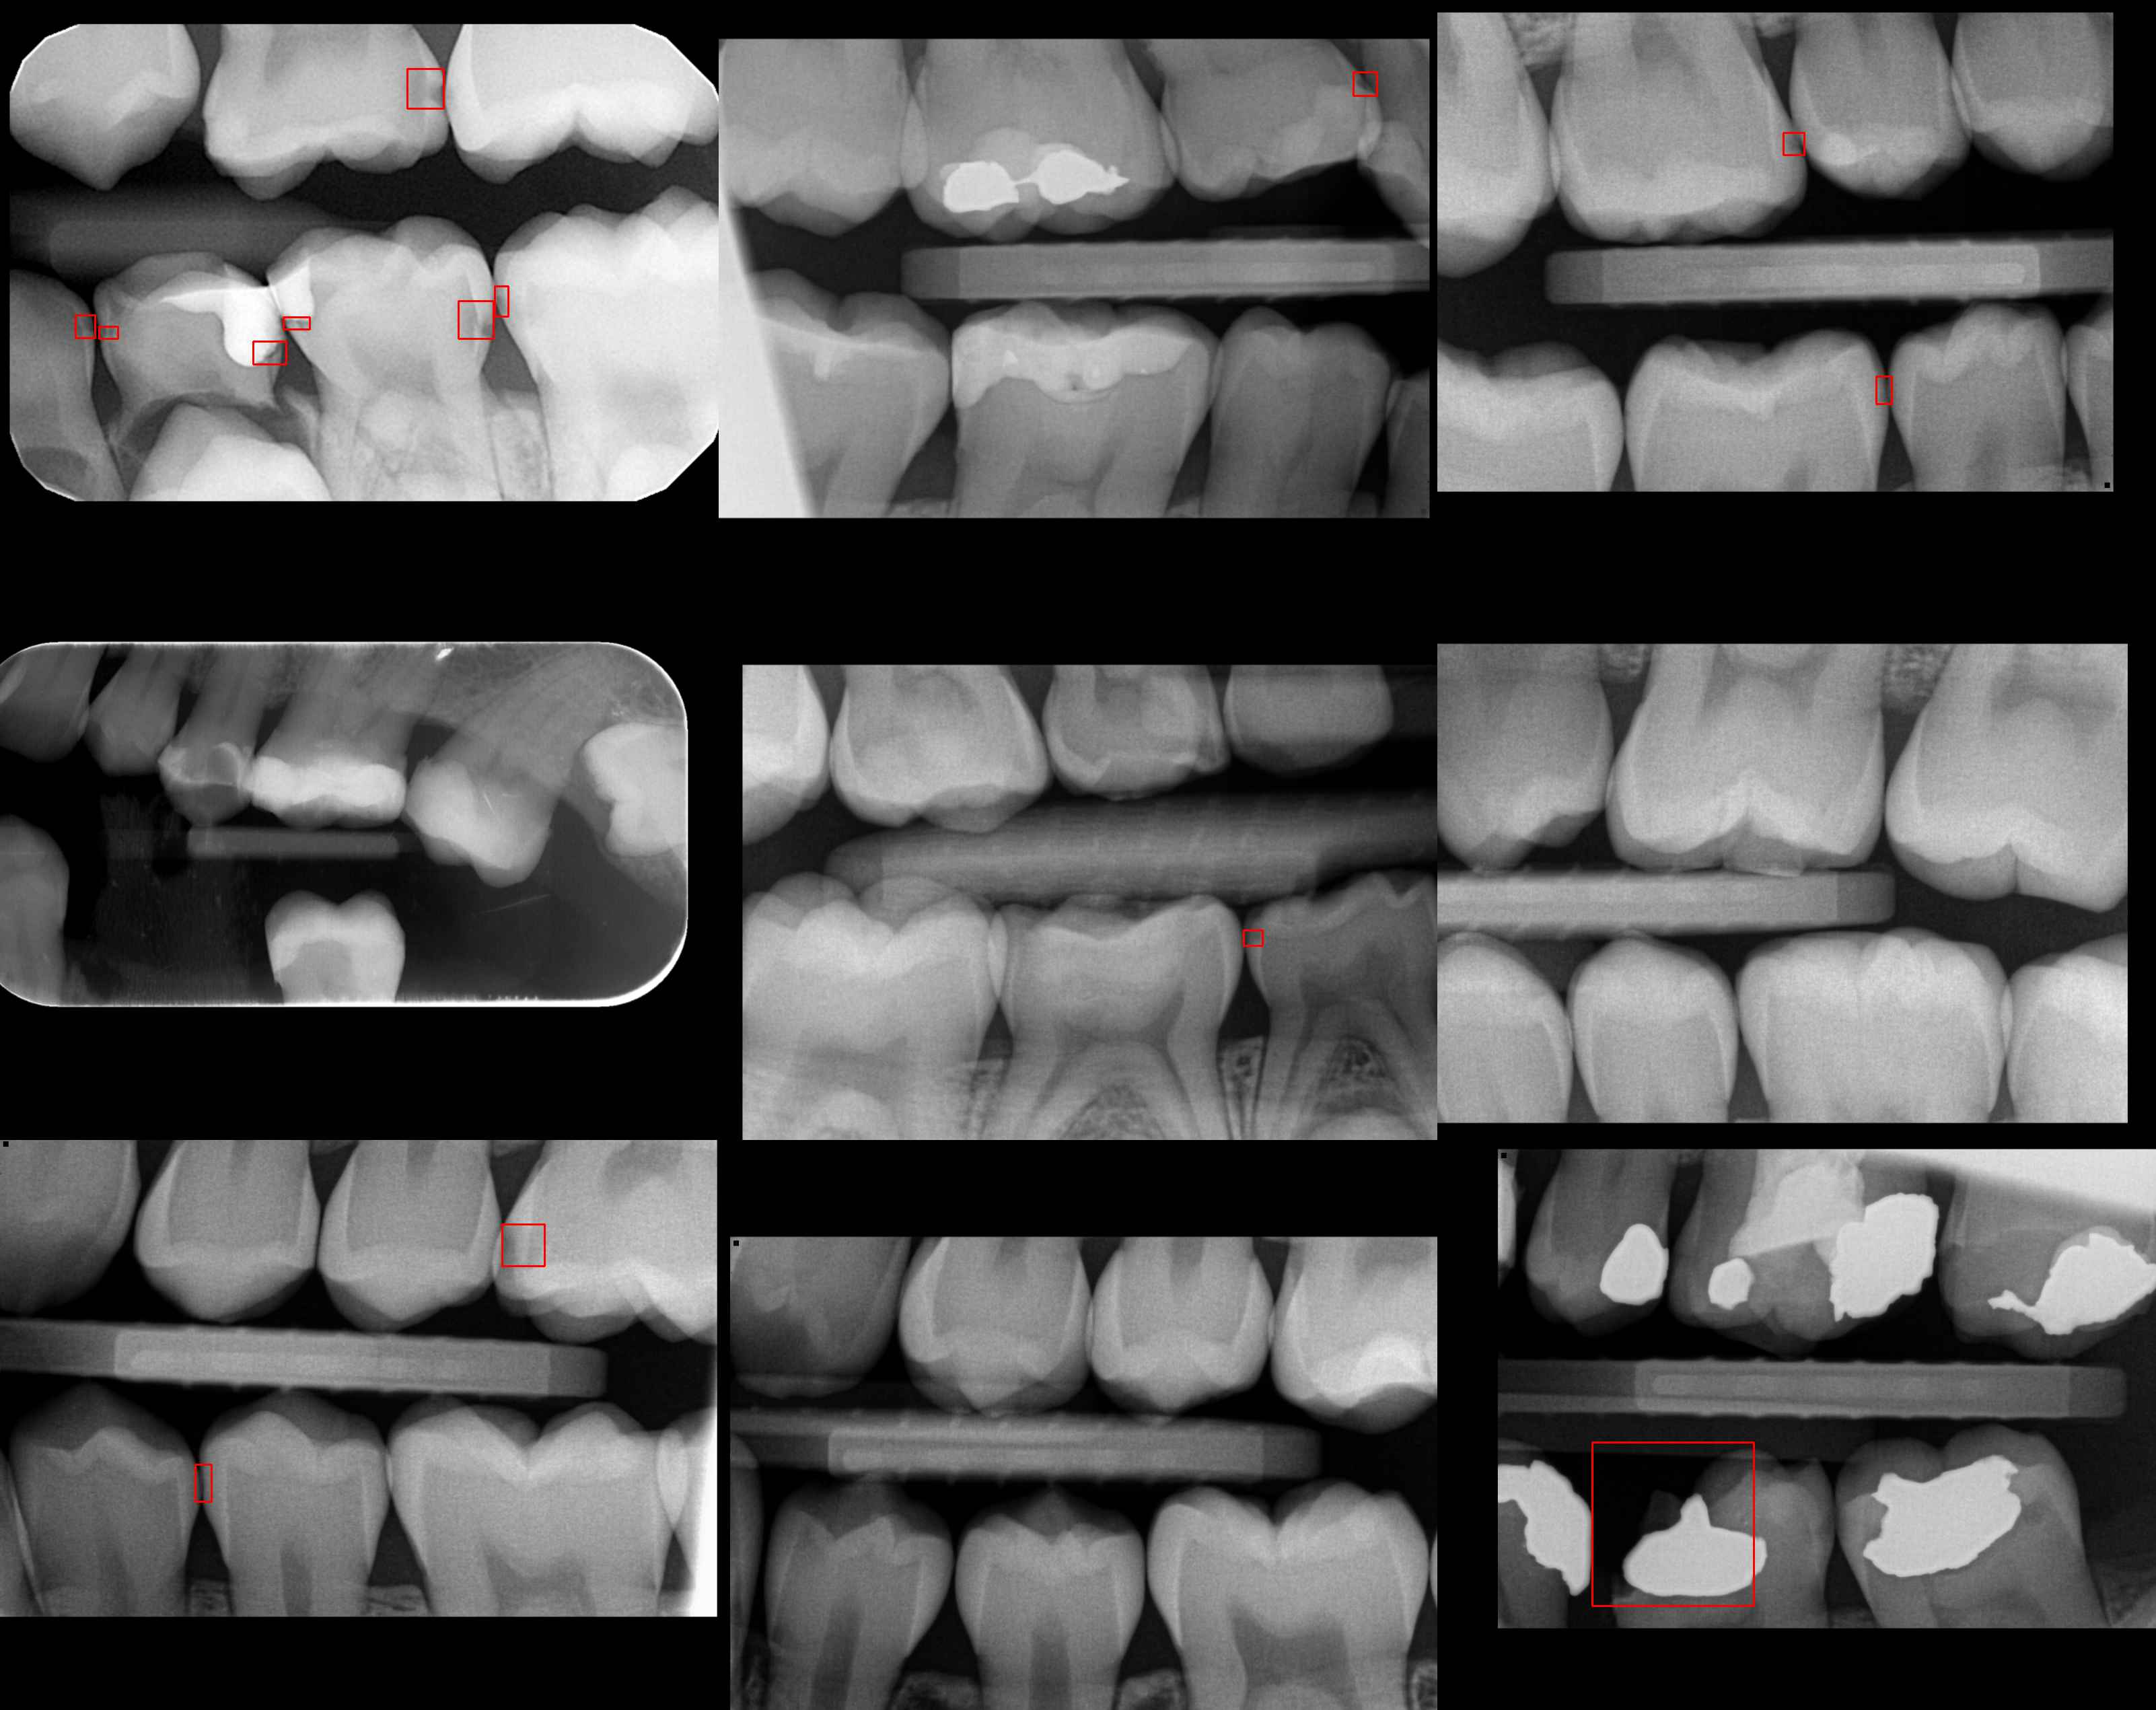
\includegraphics[width =0.8\linewidth]{images/translate.jpg}
    \caption{Translation applied}
\end{figure}
\begin{figure}
    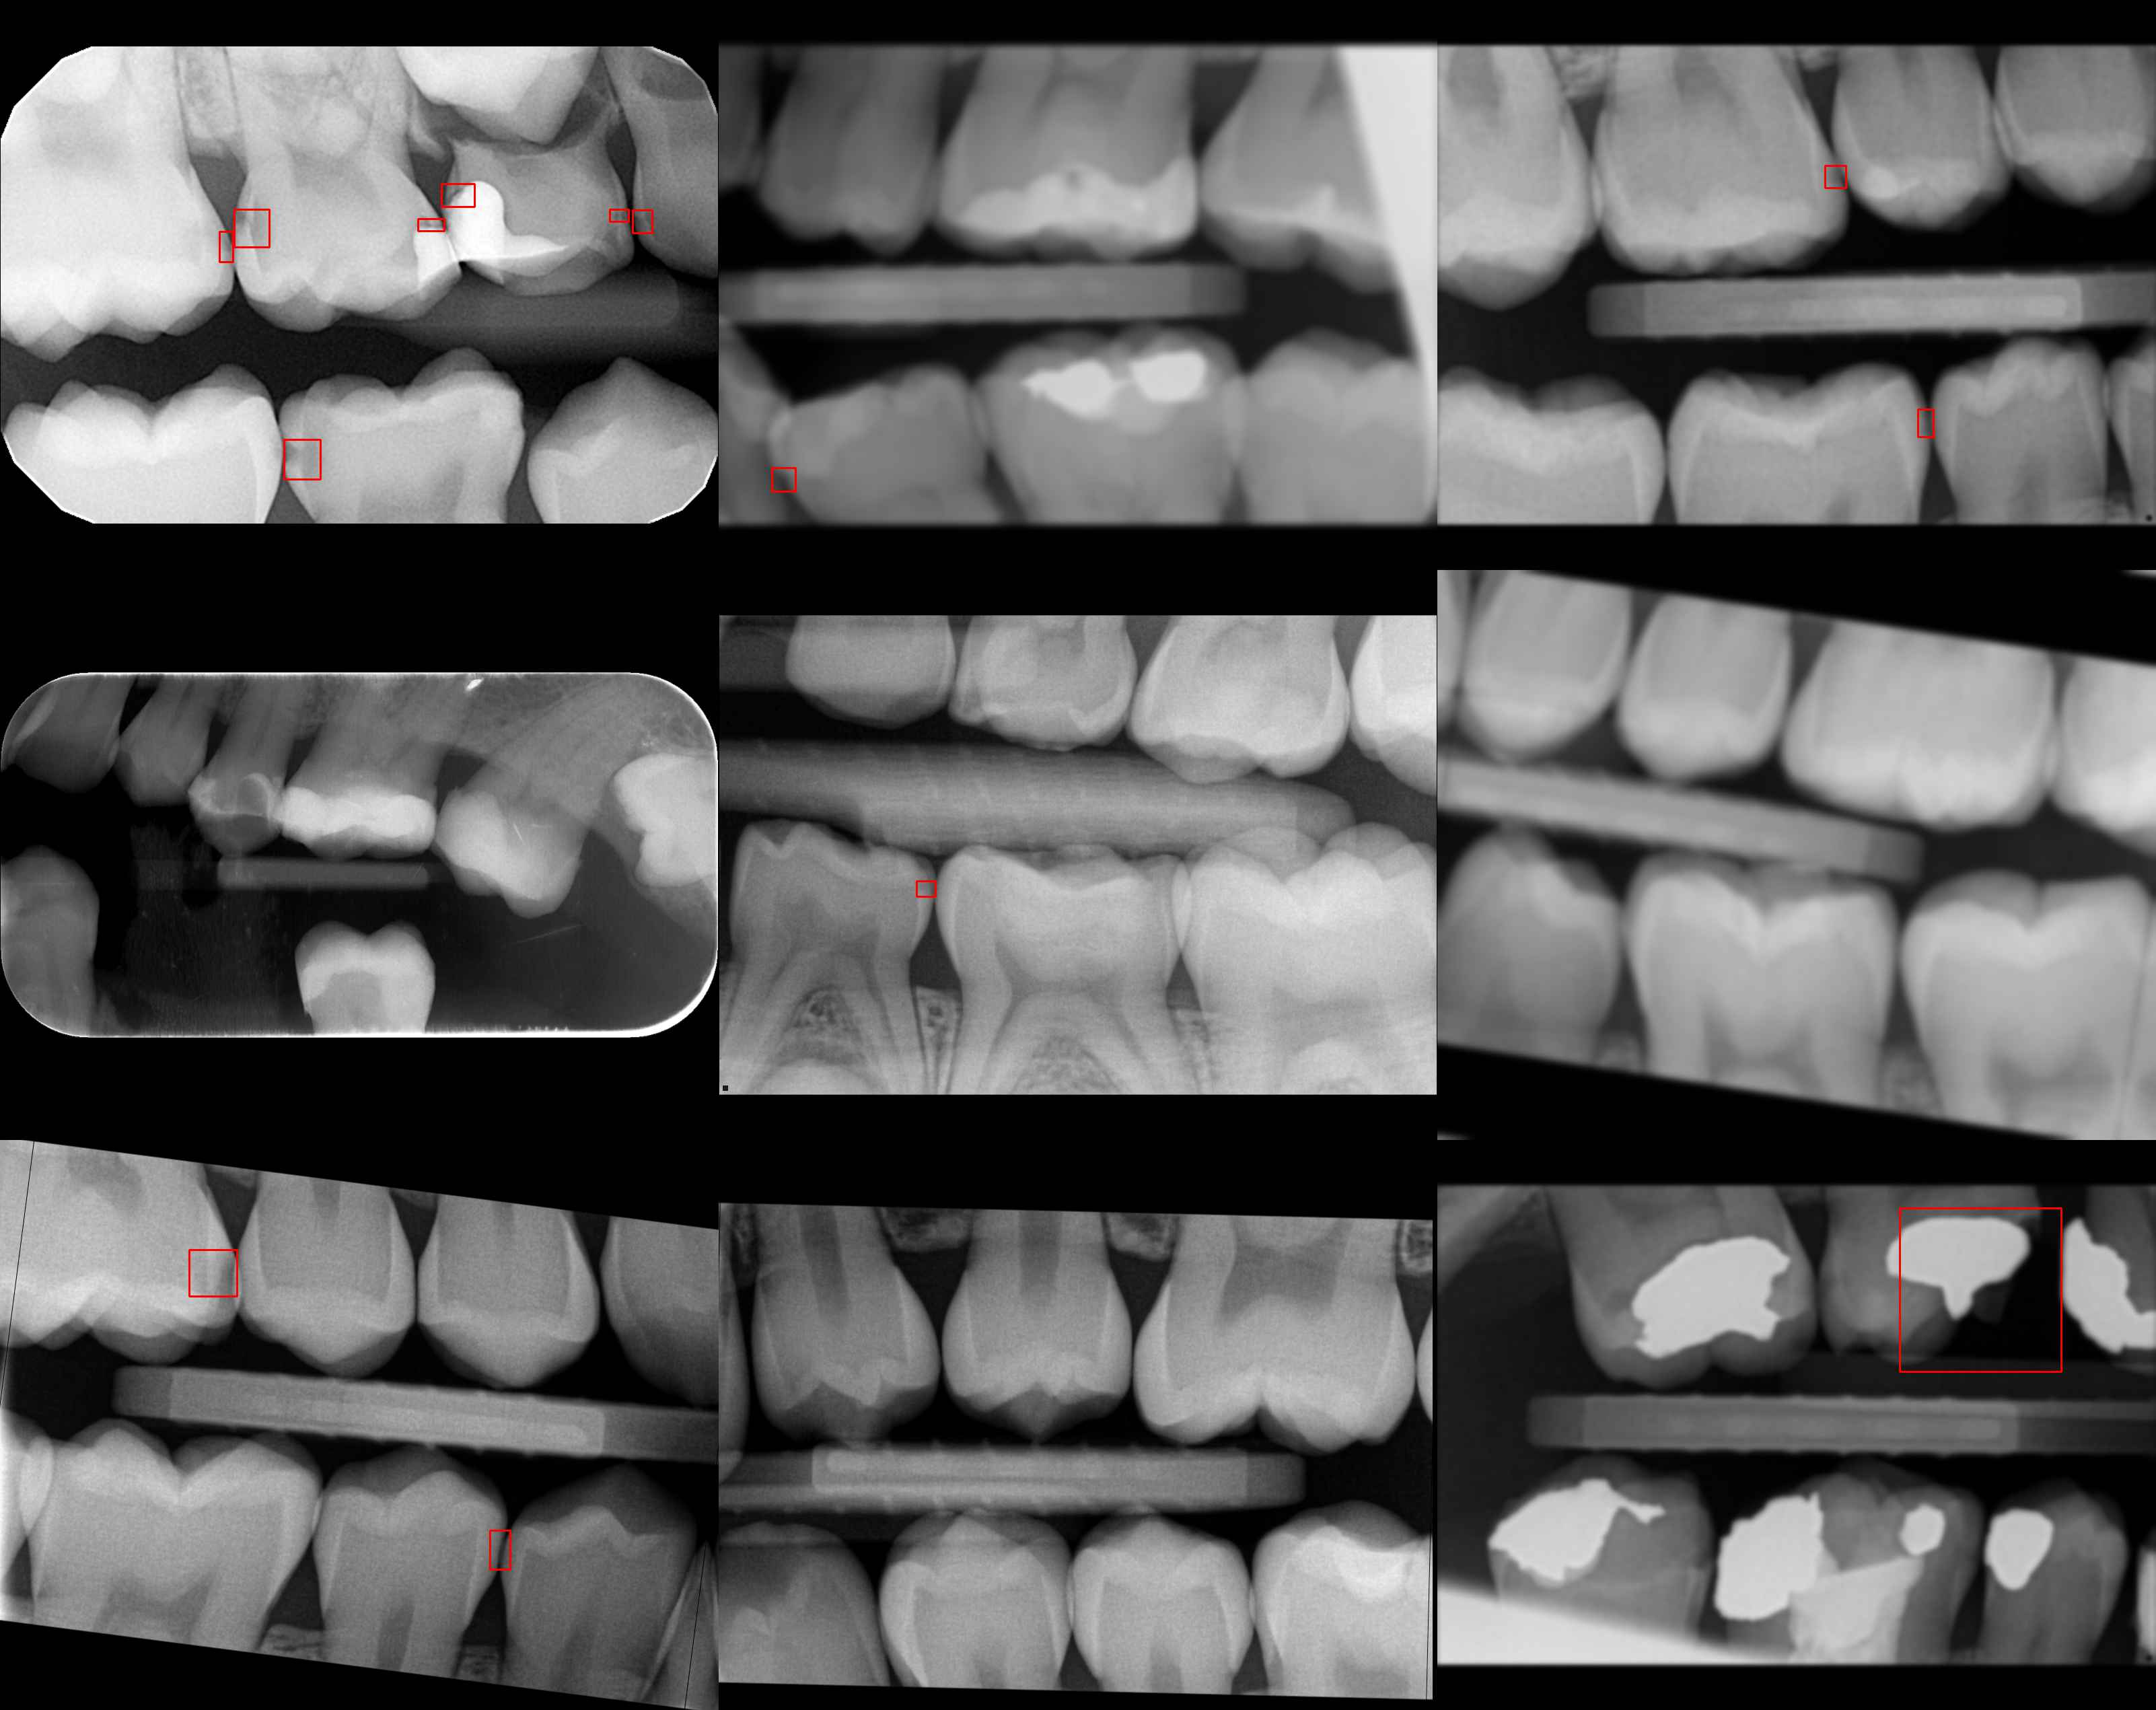
\includegraphics[width =0.8\linewidth]{images/all_transf.jpg}
    \caption{The whole augmentation pipeline applied}
\end{figure}


% \begin{figure}[h]
%     \centering
%     \begin{subfigure}[b]{\textwidth}
%         \includegraphics[width=1\linewidth]{}
%         \caption{}
%     \end{subfigure}

%     \begin{subfigure}[b]{\textwidth}
%         \includegraphics[width=1\linewidth]{}
%         \caption{}
%     \end{subfigure}
%     \caption{}
%     \label{}
% \end{figure}